\Chapter{The Building of the House}{Glyn Court}

First, one must try to imagine the village as it was early In 1914 (Figure \ref{fig:Map}) - a road curving past the station, down to the stream, and up the ramp the other side, much as today. The coming of the mineral railway had made very noticeable alterations in the landscape of this little corner, for the line ran straight down the side of the property and virtually under the window of the cottage. Its construction posed quite a problem, for the road had always run across the flat water meadow by the stream and then made a short sharp curving ascent to the cottages and chapel. In order to gain the necessary height a long sloping ramp had to be built over the top of the old road. The edge of this road can still be seen protruding from beneath the ramp - the tunnel has not yet been filled in. Traffic consists of an occasional horse and cart. The only car in the neighbourhood is owned by Count Hochberg of Croydon Hall, but as he has just gone back to Germany it is unlikely that we shall see it. The cottages in the village are rather shabby and the inhabitants do not look very prosperous. At the top of the ramp, we pass a little group of three cottages. These are occupied by two old ladies, Rhoda and Annie. Although the cottages appear low from the road which has been raised a few years earlier the interior is even lower, for it is necessary to descend three steps to the room from the front door. The lowest cottage, the one at the end which still survives, has suffered similarly from the raising of the road, and light in the main living room window has been completely blocked out by the bridge. To make matters worse, it has been damaged by fire. Instead of demolishing the remains, William is rebuilding the cottage on the foundations of the old one, the former living room now becoming a cellar. This no doubt accounts for the extraordinary shape of the place - a section from a large wedge with not a single right angle anywhere in it. As far as can be surmised the foundations date from the seventeenth century. Next to the cottages and on a higher level, there is a large field hedge running up at right angles to the road, shielding the \quotemark{drang} - a narrow path leading out at the side of the two tiny cottages.

\begin{figure}
     \includegraphics[width=1\textwidth]{figures/WashfordMap1910}
     \caption{A map of Washford, circa 1910}
     \label{fig:Map}
\end{figure}

\begin{figure}[p]
     \includegraphics[width=1\textwidth]{figures/Washford1900s}
     \caption{View of Washford from Trowden Copse, circa 1900. The West Somerset Mineral Railway can clearly be seen in the centre of the photo.}
     \label{fig:WashfordView}
\end{figure}

\begin{figure}[p]
     \includegraphics[width=1\textwidth]{figures/WashfordGarden1900}
     \caption{View of Washford, taken from the field to the rear of Hill Head House, circa 1920}
     \label{fig:GardenView}
\end{figure}

\afterpage{\clearpage}


Then there is a high wall with an orchard visible above it. The front of the orchard, facing the road which is not made up, is bounded by a sturdy wall, the top of which is finished off with those alternate standing up and flat stones so typical of this part of Somerset, and known as cap and gap. It is not a particularly attractive finish but is utilitarian, and has a certain unity in that it continues, more or less right through the village on both sides of the road. We must stop at the gate of the orchard for we have arrived at Mr Bellamy's. The orchard belongs to him, as do the cottages, a well built stable, wash-house and a couple of stone privies and pigsty. Mr Bellamy carries on his business in the bakehouse, turning out batches of sweet-smelling bread from his crude but effective oven. This is heated by the laborious method of burning bundles of sticks (faggots) inside it and then raking out the ash. In the house, his daughter, Mary, and Ada are busily occupied in running the Post and Telegraph office - a very important place in the village, patronised by everyone, including the gentry.

James Bellamy is getting on in years and is handing over his business to Henry Chilcott. He has sold part of his land to William Court who intends to marry and build himself a house. The damaged cottage is to be rebuilt to house the baker and his family who will pay rent of 5/- per week to William - an arrangement which will continue for nearly 60 years. One threatening cloud on the horizon is to grow increasingly larger and cast its shadow over at least one of these projects. Unknown to James Bellamy, William and Ada and the other personages we see moving about in this little scene, the Kaiser's war is to cause considerable deferment of their plans. When the war does break out in August of the same year, everything has to wait and Ada patiently puts off her wedding plans with William until it is over. Even then it is another two years before William, who is now 44, and spurred on by the loss of his favourite sister, Tilly, finally makes up his mind to marry.

The burning question for William and Ada was how to raise enough money to start actually building the house. In 1920 it was a fairly unusual situation for folk of their social class to attempt such a project and 95\% mortgages were a concept which had not yet been imagined. Also, both had a very deep dislike almost amounting to fear, of borrowing money. However, borrowing it had to be, from the bank and not from a building society. The money borrowed, amounting to £800 in all, would mainly be used to pay for materials as William would do a large part of the construction work himself; stone was cheap and not far to bring - while slate could be obtained from the ancient quarry of Treborough, a few miles up the valley. Transport costs were minimal, and the stone came virtually free of charge, the only payment exacted being 1/- duty on each cartload that was removed from the quarry opposite the farm. Timber also could be had locally, and William never lost an opportunity of acquiring pieces of wood which others had thrown away, or purchasing second-hand bargains. Of course, the sheer manual labour of dressing the stone, carting it and unloading and so forth could not possibly be undertaken by one man working alone, and William did enlist the assistance of at least one mason, now an old man in his eighties still living in the village.

\begin{figure}[p]
     \includegraphics[width=1\textwidth]{figures/HillHeadHousePlans1}
     \caption{Original drawings of the house (Part 1). Produced as part of the planning application submitted by William Court in 1922.}
     \label{fig:HousePlans1}
\end{figure}

\begin{figure}[p]
     \includegraphics[width=1\textwidth]{figures/HillHeadHousePlans2}
     \caption{Original drawings of the house (Part 2). The original planned footprint can be seen for the house, highlighting the single-storey shop.}
     \label{fig:HousePlans2}
\end{figure}

\afterpage{\clearpage}

Building a house was an operation which even in 1920 was not to be accomplished without a modicum of official approval. Before commencing any new \quotemark{development} as we have learnt to call it, a plan had to be drawn and submitted to the council, for though prosperity as we have come to know it had not arrived with its wholesale consumption of open fields, there was a sufficient amount of new building going on to warrant some sort of control. We still have this drawing and very interesting it is William must have spent a good deal of time planning his house, for the finished version correspond remarkably well with the original design (Figure \ref{fig:HousePlans1}) . The one major difference is that the shop was originally intended to be a single storey structure joined to the house on one side. When he came to build, this part, however, William decided to continue the walls upward over the shop end square off the total design of the house. Perhaps he felt dissatisfied with the rather lop-sided effect that the shop gave to the building -in any case the materials cost so little that it was not so very much more expensive to build on up and construct a gable to correspond with the one on the either side of the house. Problems inevitably arose, however, and he must soon have found the additional cost of all the extra materials heavier than planned. This probably explains why for fifty years the windows at the back of this side of the house were glazed with odd panes of glass, some clear, some opaque, some reeded. The frames too were odd sizes and presumably oddments acquired from junk heaps. One unexpected benefit of the fire in 1971 (Chapter 18) was that the firemen smashed the glass panes most decisively so that at last I was able to, get rid of these ugly windows. No one shed any tears over that loss.

The plan was drawn, approved, and the next step was simple - William pegged out the site himself and started to dig the foundations. When they rose a suitable distance above ground level the damp course was laid - a course of Treborough slate, clearly visible against the warm red sandstone.

Drains were presumably connected, up at an early stage, but as the building regulations of 1920 did not insist on plans of drainage, there is no record of the exact location of our sewer outfall. The only clue we have is a, distinct diagonal mark which appears on our lawn in time of drought as a set of tramlines. Where the pipes go after they leave the lawn is a mystery that will probably never be solved, except by an unusually intelligent mole.

As soon as the house was habitable, William and Ada moved into it, some time in 1922. The removal must have been a major operation, as not only did they have to establish themselves and get the feel of a new home, but the post office and business had to be installed as well. Miss Bellamy relinquished her superintendency of the Washford Post Office and after fifteen years of apprenticeship Ada now became the postmistress. This was a serious responsibility and one which I think gave her great satisfaction. The hours were long but the pace of life relatively calm and quiet, and it was pleasant talking to the villagers, and helping them to sort out their problems. At about the same time William had formally relinquished the situation of Postmaster at Roadwater and handed it over to his sister Selina - a transaction which was suitably blessed by the Head Postmaster. Selina would not be able to deal with the full scale boot and shoe store and repair service on her own, so William was faced with the not inconsiderable task of transferring all the paraphernalia and much of the stock to the new premises at Washford. I am heartily convinced that he thoroughly disliked the having to change everything, and can easily imagine him affirming that this would be the first and last time that he would ever move house. Some of the items were heavy, and no doubt it took numerous journeys to Roadwater to fetch everything. The \quotemark{James} motorcycle was now obsolete and he soon progressed to a motor car - one of the few in the village - a Calcott tourer with collapsible hood.

Not the least of the problems connected with the removal of the business was where to have the workshop. Shoe repairing is a trade requiring plenty of space for the sheets of leather, work bench, sewing machine, stock of tacks, nails, heels, and so forth. The only suitable building was the wash house. It was not really large enough for the purpose and in order to get to it customers would have to walk right across the back of the house and round the corner into the garden, but it would serve for the time being.

The shop was a large and commodious space, but as to begin with there was no equipment to go in it, William had to make everything that was necessary, knocking up shelves and a counter out of odd pieces of wood. This part of the building was never really finished off properly, partly because of the lack of money, and partly because it was in such constant use once the post office and store began to operate from there, that there was little opportunity for doing anything more to it. The walls were plastered, received a hasty coat of whitewash and after that were never again painted. The shortage of money led to the ceiling being finished off with laths of thin plywood, a cheaper and quicker finish than plastering. The unexpected effect of this was that the wood had the effect of creating a sound box over the post office area so that every sound made above was heard and magnified through the thin floorboards. This used to cause quite a few problems when some years later my children used to take it into their heads to have noisy games in the room above, jumping from the high box spring bed on to the floor with devastating effect. Poor Granny used to get very upset at this, I think she expected the \quotemark{customers} to complain. Unfortunately, as I had not grown up in the environment, I was never able to induce in myself the state of quasi-religious veneration for the Post Office and in any case it gave the pensioners something to talk about!



During the building of the house William and Ada had been living with Miss Bellamy at the Post Office over the road (Figure \ref{fig:PostOffice}). It was not a very happy arrangement and understandably enough, they were longing to get into their own home at the very earliest opportunity. Ada often used to say how she never missed going across to the house one single day all the time it was being built. As soon as one or two rooms were habitable, they moved in, surrounded by bricks, plaster, cement, tools and all the appurtenances of an unfinished building operation. Many doors and windows had not yet been made, and the fireplace in the big room was not to be completed for another eight years. However, it was four walls, and although we have no record of their feelings it must have been a very happy day when they began to camp out in the newly plastered rooms. The empty unfinished spaces must have seemed rather eerie and hollow and the focal point of the house very quickly became the sheltered, sunny living room at the back, with the adjoining scullery, or back kitchen. The fire in the living room, always known as the kitchen, heated the water, a rare luxury for them, who had never enjoyed more than a cold tap. It was one of those rather fearsome black stoves, with two ovens and hobs for boiling over the fire - a very functional arrangement which one still finds as a standard fitting in many houses in the North where coal is cheap. The stove was not particularly economical, but for a long time it was the only cooking or heating facility in the house. Also, it must have been well made as it lasted for nearly forty years.

\begin{figure}[p]
     \includegraphics[width=1\textwidth]{figures/HillHeadHouse}
     \caption{A photo of Ada, Glyn and William outside the newly constructed house. The shop can be seen to the left part of the property.}
     \label{fig:HillHeadHouse}
\end{figure}

\begin{figure}
     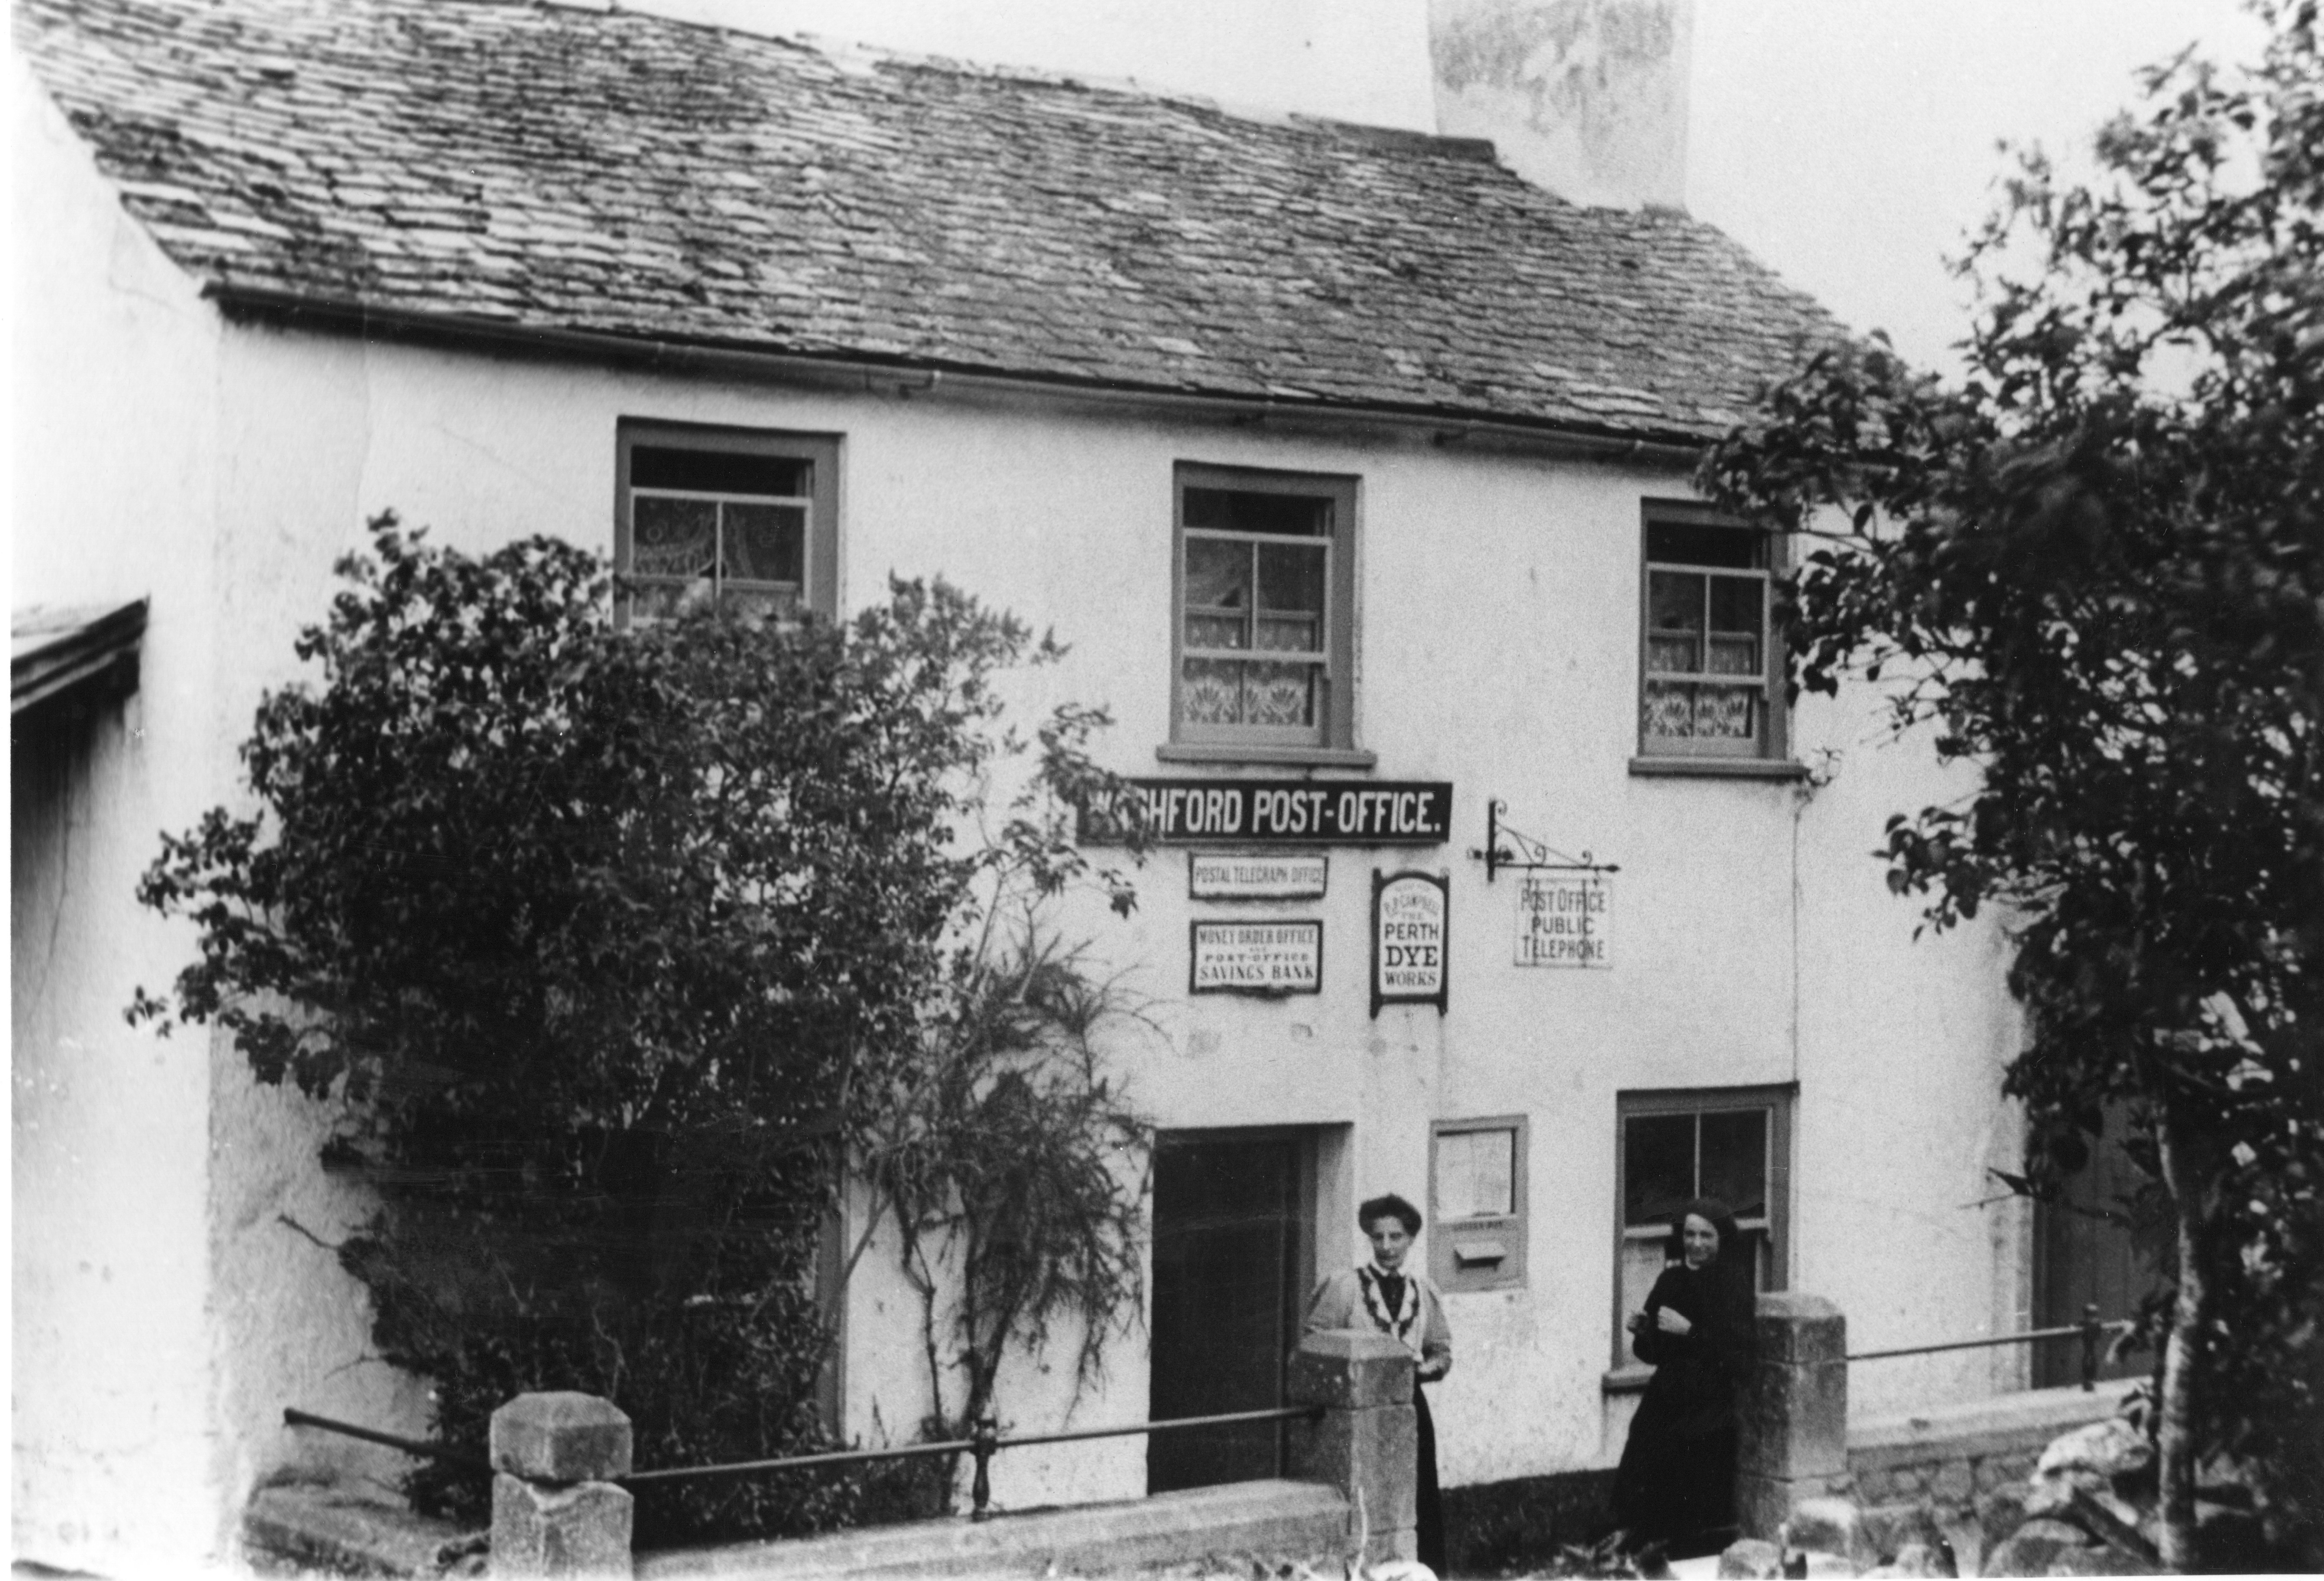
\includegraphics[width=1\textwidth]{figures/OldPostOffice}
     \caption{A photo of the Old Post Office in Washford, before being relocated to Hill Head House}
     \label{fig:PostOffice}
\end{figure}

\begin{figure}
     \includegraphics[width=1\textwidth]{figures/Cottages}
     \caption{A view of the cottages previously built on the land. The two smaller cottages were demolished in the 1920s, and were located where the driveway is now. The photo was taken around 1925, as the eaves of Hill Head House can be seen in the top right of the photo.}
     \label{fig:Cottages}
\end{figure}

\afterpage{\clearpage}

All the woodwork in the house was made by William - that is to say, all skirting boards, doors, window frames, and ornamental exterior woodwork. Altogether, the house has nineteen doors and about twenty windows, some of which are large bays with up to fourteen lights in them, so you will see that he had a good, excuse for not doing the gardening as well. The \quotemark{best} part of the house - i.e. the front, North side, was destined to receive the cherished oak that he prized so much. Many of the pieces had been saved from old buildings or even rubbish heaps, and every panel, every door frame, every carved knob (and there are many) was worked by hand. As any amateur handyman will know, oak is hard as iron, and consequently driving in screws or fixing hinges becomes a major task. An amusing discovery that we made when trying to cure a door that persisted in lurching at an undignified angle, was that it was held on by only two screws, one at the top and one at the bottom. Fortunately the electric drill has arrived on the scene to take the backache out of this sort of work, and the door now boasts far more screws than it ever knew before, Similarly, several of the windows had never been opened, which annoyed me as I like fresh air, and the reason soon became apparent - some had no stays or catches on, others had not even any hinges. One day we will catch up with all these little jobs but it takes persistence and is also very expensive.

I have mentioned my father-in-law's love of oak - this had no doubt been impressed on him as a young man when, abandoning the family tradition of bootmaking, he went to train as a carpenter's apprentice. His wages soon rose from 6d to 6 pence and one farthing per hour, 1/4 d more than the ordinary carpenters, as he had a natural flair for the work and soon became skilled. To the end of his life he could not bear to throw away a piece of wood, and we have had ample cause to bless his forethought. Looking round for gateposts in our enormous garage where most of the old wood was stored we found two long beams- resting across the traverses which support the tin roof. They were of oak and we had been looking at them for years without realising what they were. Much of the old wood was virtually useless of course, and only fit for the bonfire. As my old gardener remarked \quotemark{Tis old as Adam, Madam!}

We have now been living here for seven years and I think that we have reduced the wood to manageable proportions - although we shall not have to look very far for kindling sticks for ten years at least. 

\Flourish	 
 
People often ask us why the corrugated iron monstrosity, known as \quotemark{the Garage} is so enormous. The reason is that when delivery of the mail by motor vans first started, space had to be found to keep the two vehicles which were based at Washford. These vans were very high and much larger than the modern ones. One was a Morris Cowley, one an Oxford. They had calor meters on the front of the bonnet and regularly used to boil when going up steep hills. William had to build a garage for the vehicles as cheaply as possible, and threw this enormous lean-to roof up against the wall of Butcher Shepherd's slaughterhouse next door. Relations were quite strained for a while, as the building operation blocked out the light from one of the butcher's windows. Nor was it a straightforward task, as the ground sloped away at an inconvenient angle, so literally tons of soil had to be dug out to create the necessary level space. We have never quite made out what happened to all this soil. As a finishing touch to this unlovely but useful creation, the Garage, William constructed a sliding door. It still slides perfectly after forty-three years, but is so heavy that we rarely bother to close it. On the front of the door, still faintly visible, is the legend:

\begin{center}
W, G. Court\\
Garage
\end{center}


Glyn remembers his father painting it on and the pleasure that he derived from making the letters appear to lie flat on the corrugated material. Frequent interruptions to the work had to be made before William was satisfied with the perspective.

In one corner of this edifice, (which when tidy will comfortably hold four cars) stands the 1932 Austin 10 in which my parents-in-law drove around until William's death in 1953. The car then passed to us and we drove it really hard for another five years. We were living in Yorkshire at the time so the 200 mile journey must have taxed the engine considerably. She never broke down however. The previous car, a Calcott, was not preserved, I cannot think why not. It would have been valuable if it had. Black mark.

Above the Austin, there is a further cobwebby extension, looking more than a little improbable perched high up seemingly in the heavens, like a strange attic, full of mysterious pieces of twisted metal. The illusion of height is given by the steep rise in the ground level at the back of the garage, and a close examination reveals a heap of very old bicycles. The one at the bottom looks as if it might be pre 1914 vintage. We are putting off taking the bicycles out until we have the time and money to deal with them properly. Meanwhile they will probably not deteriorate much more in a mere ten years or so than they have in the last thirty, forty or even sixty. Ten years at Washford, as I have come to learn, is a very short space of time indeed.

The rest of the garage proved a fruitful quarry when we were having one of our first turn-outs. Several advertising signs from the 1920s and '30s turned up - the metalled enamel variety. The rest of the space tends to get filled up with unwanted pieces of furniture, and boxes of burnt books left over from the fire.

The days of the Garage are numbered now as rust is making progress and quite a lot of rain finds its way through the roof, but let it not be said that its life and work have not been recorded for posterity!
